\documentclass[specialist,
               substylefile = ../spbu.rtx,
               subf,href,colorlinks=true, 12pt]{disser}

\usepackage[a4paper,
            mag=1000, includefoot,
            left=3cm, right=1.5cm, top=2cm, bottom=2cm, headsep=1cm, footskip=1cm]{geometry}
\usepackage[T2A]{fontenc}
\usepackage[utf8]{inputenc}
\usepackage[english,russian]{babel}
\ifpdf\usepackage{epstopdf}\fi

% Использовать полужирное начертание для векторов
\let\vec=\mathbf

% Включать подсекции в оглавление
\setcounter{tocdepth}{2}

\usepackage[defaultmono]{droidmono}
\usepackage[T2A]{fontenc}
% \usepackage{csquotes}

\usepackage[intlimits]{amsmath}
\usepackage{amsfonts}
\usepackage{amssymb}
\usepackage{amsthm}

\usepackage{algorithm2e}
\usepackage{graphicx}
\graphicspath{ {../media/} }
\usepackage{color}

\usepackage[fixlanguage]{babelbib}
\selectbiblanguage{russian}

% \usepackage{natbib}
% \usepackage[style=numeric]{biblatex}
% \addbibresource{biblio-u.bib}

\usepackage{hyperref}
\newtheorem{theorem}{Теорема}
\newcommand{\ev}{\mathrm{E}}
\newcommand{\vfi}{\varphi}
\newcommand{\prob}[1]{\mathsf{P}\left(#1\right)}
\newcommand{\R}{\ensuremath{\mathbb{R}}}
\newcommand{\Tau}{\ensuremath{\mathcal{T}}}
\newcommand{\GothB}{\mathfrak{B}}
\newcommand{\norm}[1]{\left\lVert#1\right\rVert}
\newcommand{\Vhat}{\hat{V}}
\newcommand{\vhat}{\hat{v}}
\newcommand{\maxset}[1]{\max\left\lbrace#1\right\rbrace}
\DeclareMathOperator*{\argmax}{arg\,max}
\DeclareMathOperator*{\argmin}{arg\,min}

% \renewcommand\topfraction{0.85}
% \renewcommand\bottomfraction{0.85}
% \renewcommand\textfraction{0.1}
% \renewcommand\floatpagefraction{0.85}
\setlength\parindent{0pt}
\setlength\parskip{0.5em}

\begin{document}

%
% Титульный лист на русском языке
%

% Название организации
\institution{%
    Правительство Российской Федерации \\
    Федеральное государственное бюджетное образовательное учреждение \\
    высшего профессионального образования \\
    «Санкт-Петербургский государственный университет» \\
    Кафедра статистического моделирования
}

\title{Отчет по научно-исследовательской работе}

% Тема
\topic{\normalfont\scshape%
    Некоторые методы оценки стоимости американских опционов}

% Автор
\author{Миллер Анастасия Александровна}

% Научный руководитель
\sa       {С.\,М.~Ермаков}
\sastatus {д.\,ф.-м.\,н., профессор}

% Город и год
\city{Санкт-Петербург}
\date{\number\year}

\maketitle

\tableofcontents

\intro
	Задачами семестра являлись формулировка проблемы на языке тропической математики и проведение детального сравнения разрабатываемого метода с методом стохастической сетки. Первая глава посвящена переформулировке задачи, во второй представлено краткое описание метода стохастической сетки и проведён анализ преимуществ и недостатков этого метода по сравнению с разрабатываемым.

\chapter{Задача оценки американского опциона в терминах тропической математики}
	Для Американского опциона с функцией выплат $h_t\left(X_t\right)$, где $X_t$ --- состояние актива, на который выписан опцион, в момент времени $t \in \left[0; T\right]$, задача оптимального исполнения --- это задача о нахождении
	\begin{equation}\label{eq:general setting}V = \max_{\tau} \ev h_\tau\left(X_\tau\right).\end{equation}
	При дискретизации \eqref{eq:general setting} (принятии предположения о том, что опцион может быть исполнен только в некотором конечном числе моментов времени $\left(\lbrace t_i\right\rbrace_{i=0}^m \in \left[0; T\right], t_0 = 0, t_m = T$) задача обретает эквивалентную формулировку о нахождении $V_0\left(X_0\right)$ для
	\begin{equation}\label{eq:option-recursive} \begin{aligned}
		V_m\left(x\right) &= h_m\left(x\right), \\
		V_{i-1}\left(x\right) &= \max\left\lbrace h_{i-1}\left(x\right), \ev\left[V_i\left(X_i\right)|X_{i-1}=x\right]\right\rbrace.
	\end{aligned}
	\end{equation}
	В \cite{Broadie1997} были предложены оценки для $V_0\left(X_0\right)$ (см.~также \cite{Glasserman2004}). Оценка сверху:
	\begin{equation}\label{eq:upper} \begin{aligned}
		\Vhat_m^{j_1 \ldots j_m} &= h_m\left(X_m^{j_1 \ldots j_m}\right), \\
		\Vhat_i^{j_1 \ldots j_i} &= \max \left\lbrace h_i \left( X_i^{j_1 \ldots j_i} \right), \frac{1}{b} \sum_{j = 1}^b \Vhat_{i+1}^{j_1 \ldots j_i j}\right\rbrace.	
	\end{aligned}
	\end{equation}
	Оценка снизу:
	\begin{equation}\label{eq:lower} \begin{aligned}
		\vhat_m^{j_1 j_2 \cdots j_m} &= h\left( X_m^{j_1 j_2 \cdots j_m}\right), \\
		\vhat_{ik}^{j_1 j_2 \cdots j_i} &= \left\lbrace
				    \begin{array}{l l}
					    h\left( X_i^{j_1 j_2 \cdots j_i}\right), & \, \text{если } \frac{1}{b-1}\sum_{j=1, j\not= k}^b \vhat_{i+1}^{j_1 j_2 \cdots j_i j} \leq h\left(X_i^{j_1 j_2 \cdots j_i}\right), \\
					    \vhat_{i+1}^{j_1 j_2 \cdots j_i k}, & \, \text{иначе}
				    \end{array}\right. \\
		\vhat_i^{j_1 j_2 \cdots j_i} &= \frac{1}{b}\sum_{k=1}^b \vhat_{ik}^{j_1 j_2 \cdots j_i}.
	\end{aligned}
	\end{equation}
	Для обеих оценок доказана состоятельность и асимптотическая несмещённость. Обозначения $X_i^{j_1\cdots j_i}$ соответствуют путям в дереве, пример которого приведён на рис. \ref{fig:exponentialTree}.

	\begin{figure}[h]
	    \centering
		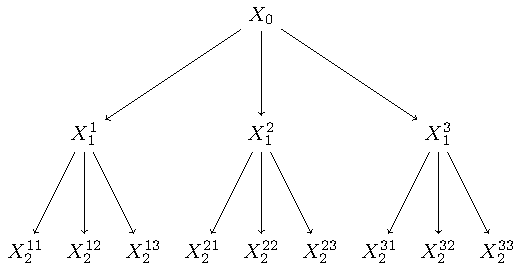
\includegraphics[width=0.8\textwidth]{exponential_tree.pdf}
		\caption{Дерево состояний актива}
		\label{fig:exponentialTree}
	\end{figure}

	Рассмотрим оценку сверху \eqref{eq:upper} на небольшом примере: $b = 3, m = 3$. Обозначим операцию $+$ как $\odot$ и $\max$ как $\oplus$. Будем также считать, что дерево состояний актива уже смоделировано и обозначим $h_i\left(X_i^{j_1\cdots j_i}\right) = h_{j_1\cdots j_i}$. Тогда
	\begin{align*}
		\Vhat_1 = h_0 &\oplus \left(\frac{h_{1}}{3}\odot\frac{h_{2}}{3}\odot\frac{h_{3}}{3}\right) \oplus \\ &\oplus\left(\frac{h_{1}}{3}\odot\frac{h_{2}}{3}\odot
					 \left(\frac{h_{31}}{9}\odot\frac{h_{32}}{9}\odot\frac{h_{33}}{9}\right)
					 \right)\oplus \\ 
		&\oplus \left(\frac{h_{}}{3}\odot
					 \left(\frac{h_{21}}{9}\odot\frac{h_{22}}{9}\odot\frac{h_{23}}{9}\right)
		\odot\frac{h_{3}}{3}\right) \oplus\\ 
		&\oplus \left(\left(\frac{h_{11}}{9}\odot\frac{h_{12}}{9}\odot\frac{h_{13}}{9}\right)\odot\frac{h_{2}}{3}\odot\frac{h_{3}}{3}\right) \oplus\\ 
		&\oplus \left(\left(\frac{h_{11}}{9}\odot\frac{h_{12}}{9}\odot\frac{h_{13}}{9}\right)\odot\left(\frac{h_{21}}{9}\odot\frac{h_{22}}{9}\odot\frac{h_{23}}{9}\right)\odot\frac{h_{3}}{3}\right) \oplus \\ 
		&\oplus \left(\frac{h_{1}}{3}\odot
					 \left(\frac{h_{21}}{9}\odot\frac{h_{22}}{9}\odot\frac{h_{23}}{9}\right)
					 \odot
					 \left(\frac{h_{31}}{9}\odot\frac{h_{32}}{9}\odot\frac{h_{33}}{9}\right)
				\right) \oplus \\ 
		&\oplus\left(
				\left(
					\frac{h_{11}}{9}\odot\frac{h_{12}}{9}\odot\frac{h_{13}}{9}
				\right)\odot\frac{h_{2}}{3}\odot\left(
					\frac{h_{31}}{9}\odot\frac{h_{32}}{9}\odot\frac{h_{33}}{9}
				\right)
			\right) \oplus \\ 
		&\oplus\left(\left(
					\frac{h_{11}}{9}\odot\frac{h_{12}}{9}\odot\frac{h_{13}}{9}
				\right)\odot\left(
					\frac{h_{21}}{9}\odot\frac{h_{22}}{9}\odot\frac{h_{23}}{9}
				\right)\odot\left(
					\frac{h_{31}}{9}\odot\frac{h_{32}}{9}\odot\frac{h_{33}}{9}
				\right)
			\right)
	\end{align*}

	В общем виде это выражение выглядит так:
	\begin{equation}\label{eq:tropic}
		\Vhat_0 = \oplus_{\gamma\in\Gamma} A\left(\gamma\right),
	\end{equation}
	где $\Gamma$ --- полное дерево глубины $m$, т.е. дерево, у всех вершин которого, находящихся на меньшем, чем $m$, расстоянии от корня, есть ровно $b$ дочерних вершин, а у вершин на расстоянии $m$ детей нет, $\gamma$ --- поддерево $\Gamma$, у каждой вершины которого либо 0, либо $b$ дочерних (примеры таких деревьев можно увидеть на рис.\ref{fig:exponential subtrees}), \begin{equation}
		A\left(\gamma\right) = \odot_{X\in\gamma}\frac{h_j\left(X\right)}{b^j}, \text{ где $j$ -- расстояние от вершины $X$ до корня.}
	\end{equation}

	\begin{figure}[h]
	    \centering
		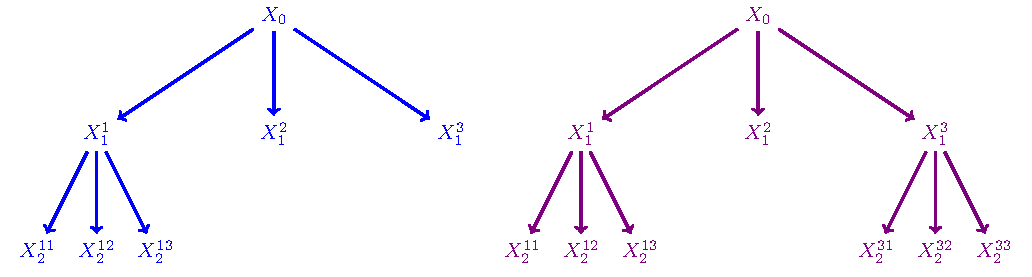
\includegraphics[width=0.8\textwidth]{exponential_subtrees.pdf}
		\caption{Примеры поддеревьев $\gamma$}
		\label{fig:exponential subtrees}
	\end{figure}

	Таким образом, мы получаем выражение для верхней оценки опциона, построенное по отдельным поддеревьям $\gamma\in\Gamma$. Если мы докажем, что для получения состоятельной оценки максимума по всем $\gamma$ необязательно подсчитывать $A\left(\gamma\right)$ для всех $\gamma$, мы добьёмся существенного снижения временных затрат.

\chapter{Сравнение с методом стохастической сетки}
	Метод стохастической сетки излагается по \cite{Broadie2004} и (неопубликованной) \cite{Kashtanov2015}.

	Метод стохастической сетки также предлагает оценки сверху и снизу для решения \eqref{eq:option-recursive}, но принцип построения оценок несколько отличается от рассматриваемых мною оценок по случайному дереву.

	Для описания состояния актива в моменты времени $t_1, \ldots, t_m$ задаются плотности распределения случайной величины, характеризующей состояние актива, в зависимости от времени, обозначим их $g_i\left(\cdot\right)$. Для каждого момента $t\in\left\lbrace t_i\right\rbrace_{i=1}^m$ генерируется $b$ точек $X_t^1, \ldots, X_t^b$ в соответствии с этой плотностью. Оценка сверху по полученной сетке определяется как 
	\begin{equation} \begin{aligned}
		\hat Q_T\left(X_i\right) &= h_T\left(X_T^i\right), \\
		\hat Q_t\left(X_i\right) &= \max\left\lbrace h_t\left(X_t^i\right), \frac{1}{b}\sum_{j=1}^b\hat Q_{t+1}\left(X_j\right) w_t\left(X_t^i, X_{t+1}^j\right) \right\rbrace,
	\end{aligned}
	\end{equation}
	где $w_t\left(X_t^i, X_{t+1}^j\right)$ --- вес, сопоставляемый переходу из $X_t^i$ в $X_{t+1}^j$. $\hat Q_0^0$ является состоятельной и асимптотически несмещённой оценкой сверху для истинной цены опциона при условии, что веса $w_t$ выбраны должным образом. Основная идея, поясняющая выбор весов, заключается в следующем рассуждении:
	\begin{eqnarray*}
	\ev\left(Q_{t+1}\left(X_{t+1}\right)\middle\vert X_t = x\right) &=& \int Q_{t+1}\left(u\right)f\left(x,t,u\right)\mathrm d u = \\
		&=& \int Q_{t+1}\left(u\right)\frac{f\left(x,t,u\right)}{g_{t+1}\left(u\right)} g_{t+1}\left(u\right)\mathrm d u = \\
		&=& \ev\left(Q_{t+1}\left(X_{t+1}\right)\frac{f\left(x,t,u\right)}{g_{t+1}\left(u\right)}\right),
	\end{eqnarray*}
	где $f\left(x, t, u\right)$ --- переходная плотность, плотность вероятности того, что актив из состояния $x$ в момент $t$ перейдёт в состояние $u$ к моменту $t+1$. Таким образом, веса компенсируют неточность, порождённую моделированием состояний базового актива без учёта траекторий его развития. Для оценок по случайным деревьям эти веса не нужны, так как плотность распределения $\left.X_{k+1}^{j_1\cdots j_{k+1}}\middle\vert X_k^{j_1\cdots j_k} = x\right.$ всегда учитывает траекторию, по которой актив попадает в состояние $X_{k+1}^{j_1\cdots j_{k+1}}$ наличием условия в правой части. Следовательно, ряд проблем, вызываемых поиском подходящей плотности $g$ и весов $w$, которые бы обеспечили отсутствие экспоненциального роста дисперсии (решение этой проблемы и предлагается в \cite{Kashtanov2015}), пропадает сам собой.

	Для построения оценки снизу моделируется ещё одна независимая траектория для базового актива, но сама оценка использует результаты, полученные при построении оценки сверху. Пусть эта независимая траектория -- это $X_0, \ldots, X_m$. Тогда правило \begin{equation*}
		\hat\tau = \min\left\lbrace t\in\left\lbrace t_i\right\rbrace_{i=1}^m \middle\vert h_t\left(X_t\right) \geqslant \hat Q_t\left(X_t\right) \right\rbrace
	\end{equation*}
	является субоптимальным правилом исполнения опциона (все моменты $\hat\tau$ являются оптимальными, но не все оптимальные моменты находятся этой политикой), следовательно, оценка
	\begin{equation}
	\hat q = h_{\hat\tau}\left(X_{\hat\tau}\right)
	\end{equation}
	является оценкой снизу для истинной стоимости опциона. Оценка $\hat q$ не имеет очевидных аналогов с оценкой снизу по случайному дереву \eqref{eq:lower}, но на её основе, возможно, получится построить оценку снизу, удобно выражающуюся через операторы тропической математики.

\conclusion
	Получена формулировка задачи как задачи поиска максимума по всем возможным поддеревьям. Такая формулировка позволяет рассчитывать на то, что при применении соответствующих теорем (предположительно, \cite{Nevzorov2000}, \cite{Zhigljavsky2008}) мы получим состоятельную оценку с меньшими временными затратами, чем в изначальном методе.

	В дальнейшем планируется разработать такую состоятельную оценку.

\bibliographystyle{ugost2008}
\bibliography{../biblio-u}
\end{document}